\begin{figure}
    \centering
    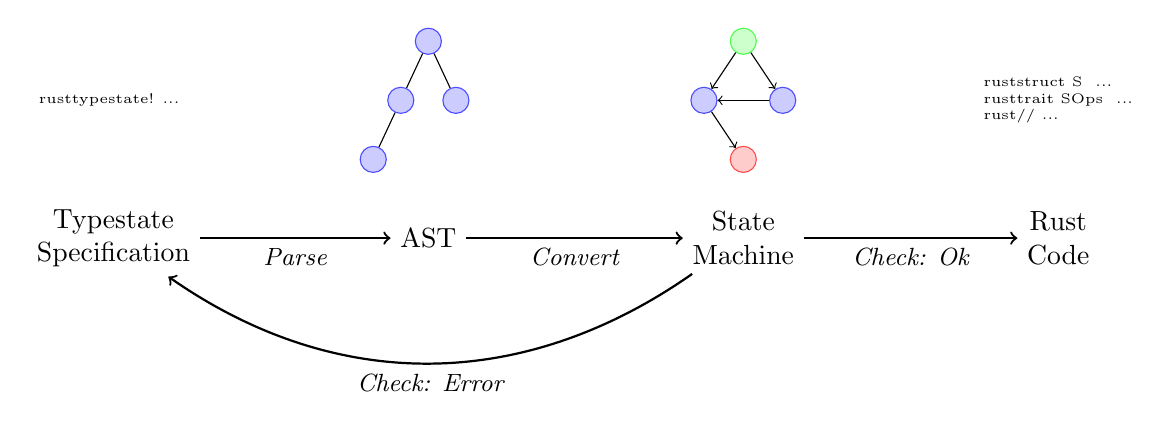
\begin{tikzpicture}
        \tikzstyle{code} = [fill=white, font=\tiny, align=left]
        \tikzstyle{phase} = [below, font=\small\itshape]

        \def\xSpec{0}
        \def\xAST{4}
        \def\xFSM{8}
        \def\xCode{12}
        \def\yLabel{-1.75}

        \node[code] (code) at (\xSpec,0) {\mintinline{rust}{typestate!{ ... }}};

        \begin{scope}[shift={(\xAST, 0.75)}]
            \tikzstyle{n}=[circle, draw=blue!70, fill=blue!20]
            \node[n] (root) at (0, 0) {};
            \node[n] (l1) at (-0.35, -0.75) {};
            \node[n] (l2) at (0.35, -0.75) {};
            \node[n] (l11) at (-0.7, -1.5) {};
            \draw[-] (root) -- (l1);
            \draw[-] (root) -- (l2);
            \draw[-] (l1) -- (l11);
        \end{scope}

        \begin{scope}[shift={(\xFSM, 0.75)}]
            \tikzstyle{n}=[circle, draw=blue!70, fill=blue!20]
            \tikzstyle{f}=[circle, draw=red!70, fill=red!20]
            \tikzstyle{s}=[circle, draw=green!70, fill=green!20]
            \node[s] (root) at (0, 0) {};
            \node[n] (l1) at (-0.5, -0.75) {};
            \node[n] (l2) at (0.5, -0.75) {};
            \node[f] (l11) at (0, -1.5) {};
            \draw[->] (root) -- (l1);
            \draw[->] (root) -- (l2);
            \draw[->] (l1) -- (l11);
            \draw[->] (l2) -- (l1);
        \end{scope}

        \node[code] (rust-code) at (\xCode,0) {\mintinline{rust}{struct S { ... }}\\\mintinline{rust}{trait SOps { ... }}\\\mintinline{rust}{// ...}};

        % \draw[->, thick] (code) -> (2.5, 0);
        % \draw[->, thick] (4.5, 0) -> (5, 0);
        % \draw[->, thick] (7, 0) -> (rust-code);

        \node[align=center] (label-1) at (\xSpec, \yLabel) {Typestate\\Specification};
        \node[align=center] (label-2) at (\xAST, \yLabel) {AST};
        \node[align=center] (label-3) at (\xFSM, \yLabel) {State\\Machine};
        \node[align=center] (label-4) at (\xCode, \yLabel) {Rust\\Code};

        \draw[->, thick] (label-1) -- node[phase] {Parse} (label-2);
        \draw[->, thick] (label-2) -- node[phase] {Convert} (label-3);
        \draw[->, thick] (label-3) -- node[phase] {Check: Ok} (label-4);
        \draw[->, thick] (label-3) edge[in=-35, out=-145] node[phase] {Check: Error} (label-1);

    \end{tikzpicture}
    \caption{
        From DSL specification to Rust code.
        First the DSL is parsed, then converted to a state machine and the properties checked
        (in the case some property is not respected, an error is issued).
        Once the properties are validated, the Rust code is generated.
    }
    \label{fig:dsl-processing}
\end{figure}